\documentclass[a4paper]{tufte-handout}
\usepackage{marvosym}
\usepackage[spanish]{babel}

\title{Sofisticación, participación y compromiso político en América Latina \thanks{Este trabajo es una versión revisada de la ponencia presentada en el VII Congreso Internacional de Comunicación Política y Estrategias de Campaña organizado por la Asociación Latinoamericana de Investigadores en Campañas Electorales (ALICE), Murcia, España, del 20 al 22 de septiembre de 2018.}
\\~\\~\\} 

\author{{\normalfont Basti\'an Gonz\'alez-Bustamante}\thanks{PRS DPhil in Politics, Department of Politics and International Relations and St Hilda's College, University of Oxford. Profesor Instructor, Departamento de Gesti\'on y Pol\'iticas P\'ublicas, Facultad de Administraci\'on y Econom\'ia, Universidad de Santiago de Chile. ORCID iD: \href{https://orcid.org/0000-0003-1510-6820}{\textcolor{blue}{0000-0003-1510-6820}}}}
\date{{\normalfont \normalsize \vspace{-1mm}University of Oxford} \\ {\LARGE \Letter} \href{mailto:bastian.gonzalezbustamante@politics.ox.ac.uk}{\textcolor{blue}{\normalfont \normalsize bastian.gonzalezbustamante@politics.ox.ac.uk}}
}%% \\~\\} % without \date command, current date is supplied

\hyphenation{Latino-america-na Elecci\'on eleccio-nes ALACIP}

%% \geometry{showframe} % display margins for debugging page layout

\usepackage{graphicx} % allow embedded images
  \setkeys{Gin}{width=\linewidth,totalheight=\textheight,keepaspectratio}
  \graphicspath{{graphics/}} % set of paths to search for images
\usepackage{amsmath}  % extended mathematics
\usepackage{booktabs} % book-quality tables
\usepackage{units}    % non-stacked fractions and better unit spacing
\usepackage{multicol} % multiple column layout facilities
\usepackage{lipsum}   % filler text
\usepackage{fancyvrb} % extended verbatim environments
  \fvset{fontsize=\normalsize}% default font size for fancy-verbatim environments

% Standardize command font styles and environments
\newcommand{\doccmd}[1]{\texttt{\textbackslash#1}}% command name -- adds backslash automatically
\newcommand{\docopt}[1]{\ensuremath{\langle}\textrm{\textit{#1}}\ensuremath{\rangle}}% optional command argument
\newcommand{\docarg}[1]{\textrm{\textit{#1}}}% (required) command argument
\newcommand{\docenv}[1]{\textsf{#1}}% environment name
\newcommand{\docpkg}[1]{\texttt{#1}}% package name
\newcommand{\doccls}[1]{\texttt{#1}}% document class name
\newcommand{\docclsopt}[1]{\texttt{#1}}% document class option name
\newenvironment{docspec}{\begin{quote}\noindent}{\end{quote}}% command specification environment

 \pdfinfo{
   /Author (Basti\'an Gonz\'alez-Bustamante)
   /Title  (Sofisticación, participación y compromiso político en América Latina)
   Subject (Tufte Working Papers)
   %% /Keywords (Capital pol\'itico, elecciones, gasto en campa\~nas, incumbencia, Chile.)
}

\addto\captionsspanish{
%%\def\refname{Bibliograf\'ia consultada}
\def\tablename{Tabla}
\def\figurename{G\'rafico}
}

%% \usepackage[numbers]{natbib}
%% \usepackage{cclicenses}

\usepackage{subfig}

\usepackage{emerald}
\usepackage[T1]{fontenc}

\usepackage{multirow} 

\usepackage{hyperref}

\usepackage{xcolor, colortbl}

\usepackage{lipsum}  

\begin{document}

\maketitle

\vspace{8mm}
\justify{\small {\bfseries Resumen:} \marginnote{{\itshape {\bfseries Palabras clave:} }}}\\~\\

{\noindent \LARGE \itshape }\\

\justify{\small {\bfseries Abstract:} \marginnote{{\itshape {\bfseries Keywords:} }}}

\vspace{8mm}
\section[Introducci\'on] {{\normalfont Introducci\'on}\footnote{Agradezco al Proyecto de Opinión Pública de América Latina (LAPOP) y a sus principales donantes (la Agencia de los Estados Unidos para el Desarrollo Internacional, el Programa de las Naciones Unidas para el Desarrollo, el Banco Interamericano de Desarrollo y Vanderbilt University) por poner a disposición los datos utilizados en este trabajo. También agradezco los comentarios de Antoine Maillet. Esta investigación fue parcialmente financiada por el Convenio de Desempeño 2018 de la Universidad de Santiago de Chile.}}

\justify{La sofisticación política, también definida como conocimiento político, tiene relación con la cantidad de temas públicos que conoce un individuo, la profundidad con la cual los maneja y su capacidad para estructurar ideas sobre estos tópicos (Luskin, 1987, véase también Cohen y Zechmesiter, 2018). La sofisticación se tiende a correlacionar de forma robusta con distintas formas convencionales y no convencionales de participación política, como también con expresiones de compromiso.}

\justify{La literatura suele asociar a la participación política convencional principalmente con actividades como el sufragio, la participación en partidos políticos y en campañas electorales (Norris, 2009). La participación no convencional, por otra parte, se vincula a la política contenciosa de corte protestatario, la cual se ajusta al repertorio de acción colectiva disponible en un momento sociohistórico específico y está delimitada por estructuras de experiencias compartidas de aprendizaje basadas en la forma de organización de la acción colectiva (Tarrow, 2012; Tilly, 2006).  En este sentido, la ciencia política y la sociología han estudiado bastante, durante el último medio siglo, cuáles son los factores sociodemográficos y actitudinales que emergen como predictores de la participación política (Almond y Verba, 1980; Verba y Nie, 1972; Verba, Nie y Kim, 1978).}

\justify{Es posible identificar variables de largo (modelo de Columbia), mediano (modelo de Michigan) y corto plazo (modelo de Rochester) que afectan la percepción y predisposiciones políticas de los individuos (Arriagada, Navia y Schuster, 2010; González-Bustamante y Henríquez, 2013). Estos modelos se adecuan al caso y al contexto sociohistórico específico. Por otra parte, también existen cuerpos teóricos complementarios, por ejemplo, Bargsted et al. (2015) identifican al menos cuatro grupos de teorías para explicar específicamente la participación electoral: (a) explicaciones sociodemográficas; (b) aproximaciones basadas en la teoría de la elección racional; (c) enfoques basados en capital social; y (d) teorías asociadas a la movilización y acceso a la información. En el marco de esta diversidad teórica, generalmente se tiende a vincular los recursos sociales, como el nivel educacional y los ingresos, con la participación y el compromiso político (Corvalán y Cox, 2013; Dalton, 1988; Schlozman, Verba y Brady, 2012; Verba, Schlozman y Brady, 1995). Variables que representan estos recursos se suelen combinar con mediciones tradicionales para aproximarse al concepto operacional de sofisticación política (Cohen y Zechmeister, 2018).}

\justify{En las encuestas de opinión la sofisticación se ha medido con distintas baterías de preguntas tradicionales, principalmente a través de preguntas de conocimiento factual. Recientemente el Barómetro de las Américas 2016/17 de LAPOP ha cambiado su forma de medir conocimiento político por una aproximación más eficiente y efectiva donde es el entrevistador el que califica el nivel de conocimiento político del entrevistado. Esta nueva medición fue validada por Cohen y Zechmeister (2018) con preguntas de conocimiento factual que se mantuvieron en el cuestionario aplicado en Colombia\footnote{Las preguntas son las siguientes: GI1. ¿Cómo se llama el actual presidente de los Estados Unidos de América?; GI4. ¿Cuánto tiempo dura el período presidencial en Colombia?; y GIX4. ¿En qué continente queda Nigeria?}.}

\justify{Este trabajo, aún en desarrollo, analiza la pertinencia y consistencia de la medición de sofisticación política como predictor de participación y compromiso político con la ola del Barómetro de las Américas 2016/17 en 19 países de América Latina (N = 31.285). Se evalúan como formas de participación y compromiso político: participación electoral, en protestas, eficacia política, identificación partidaria, interés en la política y consumo de medios.}

\justify{Este documento se estructura en tres apartados. En primer lugar, en el apartado método, se ofrece información sobre los datos, variables y los modelos econométricos que se utilizan. Luego se presentan los resultados de los análisis en tres subapartados: (a) descriptivo-correlacional; (b) modelos logísticos agrupados de un nivel; y (c) modelos de efectos mixtos de dos niveles. Finalmente, se presenta un breve resumen con los principales hallazgos y futuras líneas de investigación.}

%%%%%%%%%%%%%%%%%%%%%%%%%%%%%%%%%%%%%%%%%%%%%%%%%%

\section[M\'etodo] {{\normalfont M\'etodo}}

\subsection[Datos y medición] {Datos y medición}

\justify{Se trabaja con las encuestas del Barómetro de las Américas 2016/17 de LAPOP en 19 países de América Latina (N = 31.285). A saber, Argentina (ARG: n = 1.528), Bolivia (BOL: n = 1.691), Brasil (BRA: n = 1.532), Chile (CHL: n = 1.625), Colombia (COL: n = 1.563), Costa Rica (CRI: n = 1.514), Ecuador (ECU: n = 1.545), El Salvador (SLV: n = 1.551), Guatemala (GTM: n = 1.546), Haití (HTI: n = 2.221), Honduras (HND: n = 1.560), México (MEX: n = 1.563), Nicaragua (NIC: n = 1.560), Panamá (PAN: n = 1.521), Paraguay (PRY: n = 1.528), Perú (PER: n = 2.647), República Dominicana (DOM: n = 1.518), Uruguay (URY: n = 1.514) y Venezuela (VEN: n = 1.558).}

\justify{Se utiliza la nueva variable de conocimiento político del Barómetro de las Américas 2016/17 de LAPOP como independiente y diversas variables relacionadas con formas de participación y compromiso político como variables dependientes, tal como se detalla en la tabla 1.}

\begin{table*}[h]
  \centering
  \fontfamily{ppl}\selectfont
  %% \stepcounter{figure}
   \smallskip\noindent\small Tabla 1 \\ Operacionalización de variable independiente y dependientes \\~\\
  \begin{tabular}{c c c c}
    \toprule
    Código & Variable & Pregunta & Tipo \\
    \midrule
    \multirow{5}{*}{CONOCIM} & \multirow{5}{*}{Conocimiento político} & Usando la escala que se presenta abajo, por  & \multirow{5}{*}{Ordinal}\\
    & & favor califique su percepción sobre el nivel de  &\\
    & & conocimiento político del entrevistado: (1) &\\
    & & muy alto; (2) alto; (3) ni alto ni bajo; (4) bajo;  &\\
    & & (5) muy bajo. & \\ \midrule
    \multirow{2}{*}{VB2} & \multirow{2}{*}{Participación electoral} & ¿Votó usted en las últimas elecciones & \multirow{2}{*}{Binaria}\\
    & & presidenciales? & \\ \midrule
    \multirow{2}{*}{PROT3} & \multirow{2}{*}{Participación en protestas} & ¿En los últimos 12 meses ha participado en una & \multirow{2}{*}{Binaria} \\
    & & manifestación o protesta pública? & \\ \midrule
    \multirow{4}{*}{EFF1} & \multirow{4}{*}{Eficacia política externa} & A los que gobiernan el país les interesa lo que  & \multirow{4}{*}{Ordinal}  \\
    & & piensa gente como usted. ¿Hasta qué punto  & \\
    & & está de acuerdo o en desacuerdo con esta frase? & \\
    & & (1) muy en desacuerdo a (7) muy de acuerdo. & \\ \midrule
    \multirow{2}{*}{VB10} & \multirow{2}{*}{Identificación partidaria} & ¿En este momento, simpatiza con algún &  \multirow{2}{*}{Binaria} \\
    & & partido político? & \\ \midrule
    \multirow{2}{*}{POL1} & \multirow{2}{*}{Interés en la política} & ¿Qué tanto interés tiene usted en la política? & \multirow{2}{*}{Ordinal} \\
    & & (1) mucho; (2) algo; (3) poco; (4) nada.  & \\ \midrule
    \multirow{5}{*}{GI0} & \multirow{5}{*}{Consumo de medios} & ¿Con qué frecuencia sigue las noticias, ya sea & \multirow{5}{*}{Ordinal} \\
    & & en la televisión, la radio, los periódicos o el  & \\
    & & Internet? (1) diariamente; (2) algunas veces a  & \\
    & & la semana; (3) algunas veces al mes; (4) rara & \\
    & & vez; (5) nunca. & \\ \bottomrule
  \end{tabular}
  \\~\\ \smallskip\noindent\scriptsize Fuente: Elaboración propia con datos del Barómetro de las Américas 2016/17 por LAPOP, www.LapopSurveys.org.
  %% \caption{}
  %% \label{tab:muestra}
  %% \zsavepos{pos:normaltab}
\end{table*}

\justify{La participación electoral varía dependiendo del país, por lo cual la medición va desde la participación en 2011 a 2016, dependiendo del trabajo de campo en cada país. Por ejemplo, en Nicaragua y México se preguntó sobre la participación en las últimas elecciones presidenciales de 2011 y 2012 respectivamente. En Ecuador, Honduras, Paraguay y Venezuela sobre la participación en las últimas elecciones presidenciales de 2013, mientras que en Chile sobre la participación en la primera ronda del mismo año. En otro conjunto de países se midió la participación en las últimas elecciones presidenciales de 2014: Bolivia, Brasil, Colombia, Costa Rica, El Salvador, Panamá y Uruguay. En el caso de Costa Rica, El Salvador y Uruguay se midió la participación en primera ronda, mientras que lo mismo sucedió con Argentina y Guatemala, pero en 2015. Por último, las mediciones más recientes corresponden a Haití, Perú y República Dominicana en 2016, de los cuales los dos primeros casos fueron participación en la primera ronda de las elecciones presidenciales.}

\justify{Es importante destacar que la participación electoral tiende a presentar problemas de sobre-reporte (Corvalán, Cox y Hernández, 2015). La respuesta a esta pregunta puede ser altamente sensible al falseamiento (faking) por deseabilidad social dadas las características de la situación que se desea medir (Calderón y Ximénez, 2014; Stark et al., 2001). En este caso, la deseabilidad social puede estar asociada a una connotación moral del sufragio sin importar si el sistema de votación es obligatorio o voluntario. Sin embargo, aunque la medición de este ítem presenta una alta variabilidad dados los contextos particulares de cada país, una ventaja importante es que se controlan los riesgos del sobre-reporte ya que en todos los casos se mide participación postelectoral auto-reportada y no participación preelectoral o intención futura de voto, la cual es más propensa a la deseabilidad social (Smets y van Ham, 2013).}

\justify{También se utilizan como variables de control en los modelos econométricos sexo (Q1: 0 = mujer; 1 = hombre), edad (Q2) y zona de residencia (UR: 0 = rural; 1 = urbana). Como se utilizan modelos con distribuciones binomiales hay tres variables dependientes que se deben recodificar como binarias: eficacia política, interés en la política y consumo de medios. La primera se recodifica tomando como valor positivo las tres categorías más “de acuerdo”. La variable interés por la política considera como valor positivo las categorías “mucho” y “algo”. Por último, para consumo de medios solo se considera el consumo diario.}

\subsection[Modelos econométricos] {Modelos econométricos}

\justify{Primero se estiman modelos logísticos de un nivel (Maximum Likelihood Logit Models) con un conjunto de datos agrupado que contiene a todos los países. Los modelos logísticos buscan explicar Yi como variable dependiente binaria para la observación i (Y = 0; Y = 1). Como tienen distintas probabilidades de ocurrencia se utiliza una distribución Bernoulli para modelar Yi (Cameron y Trivedi, 2010; Greene, 2012; Long y Freese, 2014).}

\justify{Se ajusta un modelo por variable dependiente utilizando la variable independiente sofisticación política y como control sexo, edad y residencia. Adicionalmente, se agregan 18 variables dummies, una por país de las muestras nacionales incorporadas al conjunto agrupado. Se utiliza el caso chileno como categoría de referencia. Se realizan pruebas con el factor de impacto de varianza (Variance Impact Factor, VIF) asimilando la distribución Bernoulli a una gaussiana para así controlar el nivel de multicolinealidad.}

\justify{Para las regresiones logísticas se utiliza un ajuste para modelos con muestras complejas con el estimador de varianza Taylor linealizado (Särndal, Swensson y Wretman, 1992; Skinner, Holt y Smith, 1989). Se consideran los estratos de la muestra (strata), las unidades primarias de muestro (PSUs) y un factor de expansión muestral o ponderador construido especialmente para realizar comparación entre países (weight1500). Para esto se sigue el esquema de ponderación y las recomendaciones técnicas de Vanderbilt University para el uso de datos del Barómetro de las Américas.}

\justify{Para obtener el factor de expansión especial se utiliza el ponderador de cada muestra nacional y se multiplica por un indicador simple compuesto por un valor estandarizado (n = 1.500) sobre el n de cada muestra nacional. Esto asegura la confiabilidad del proceso de inferencia estadística, sin embargo, un límite es que solo resulta posible evaluar la bondad de ajuste de los modelos con McKelvey y Zavoina R2 (Freese y Long, 2006; Long, 1997).}

\justify{Posteriormente, se utilizan regresiones logísticas multinivel de efectos mixtos (Mixed-effects Logistic Regressions), las cuales contienen efectos fijos y aleatorios. Esto permite una modelación con correlación intracluster donde las observaciones se ajustan porque comparten efectos de su mismo nivel o grupo (Cebolla, 2013; Demidenko, 2004; Maillet, González-Bustamante y Olivares, 2016; McCulloch, Searle y Neuhaus, 2008; Rabe-Hesketh y Skrondal, 2012).}

\justify{Se utilizan modelos de dos niveles por cada variable dependiente: donde para una serie de M clústeres independientes, en este caso las muestras nacionales, hay también un conjunto uj de efectos aleatorios (Pinheiro y Bates, 1995; Pinheiro y Chao, 2006). En el primer nivel se modela la variable de conocimiento político y las de control, mientras que en el segundo se anida a los países. Para estos modelos solo se reporta el logaritmo de verosimilitud (Log Likelihood, LL) y los valores del criterio de información de Akaike (1973) (Akaike Information Criterion, AIC), calculado como $(-2lnL + 2k) / n$, y el criterio de información bayesiano (Bayesian Information Criterion, BIC; véase Raftery, 1995), calculado con $D2 - (n - k) * ln (n)$.}

%%%%%%%%%%%%%%%%%%%%%%%%%%%%%%%%%%%%%%%%%%%%%%%%%%

\begin{marginfigure}
  \centering
  \smallskip\noindent\small Figura 1 \\ Distribución del conocimiento político-entrevistador, América Latina 2016/17
  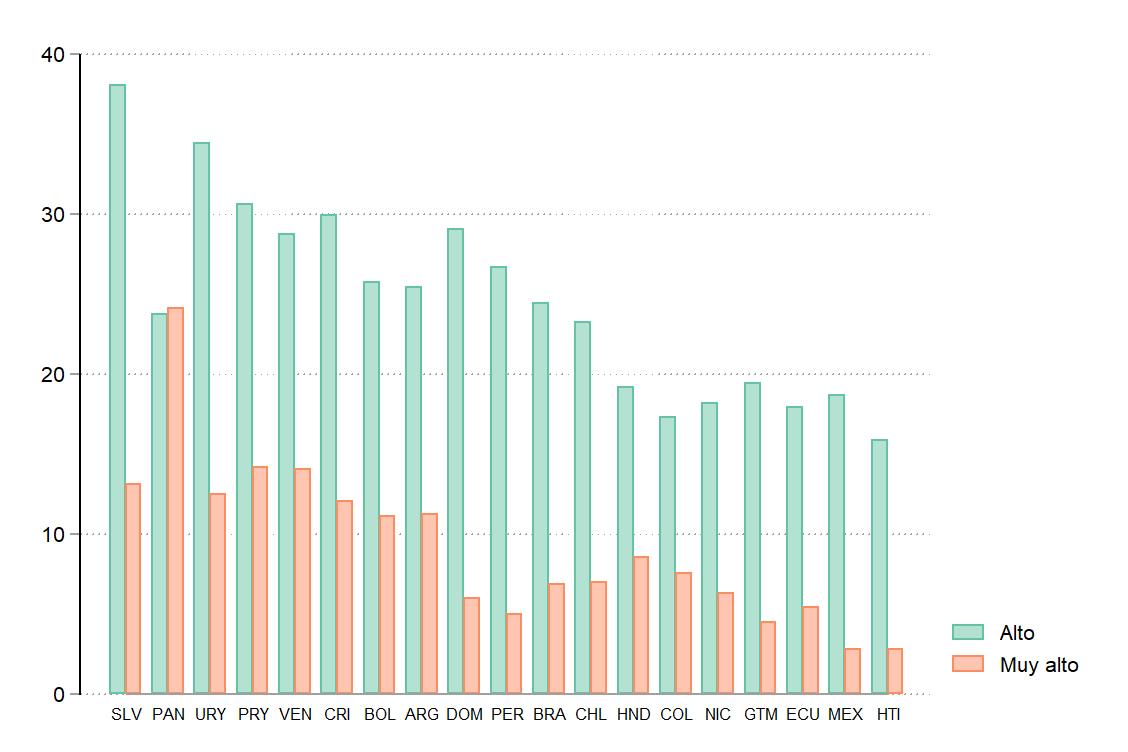
\includegraphics[width=.95\linewidth]{figures/conocim}
  %% \caption{}
  %% \label{fig:fullfig}
  \\ \smallskip\noindent\scriptsize Nota: Estimaciones puntuales ponderadas de la evaluación del conocimiento político realizada por el entrevistador. Solo se grafican las categorías “alto” y “muy alto”.\\
  Fuente: Elaboración propia con datos del Barómetro de las Américas 2016/17 por LAPOP, \href{https://www.vanderbilt.edu/lapop/}{\textcolor{blue}{www.LapopSurveys.org}}.
\end{marginfigure}

\section[Resultados] {{\normalfont Resultados}}

\subsection[Análisis descriptivo y correlacional] {Análisis descriptivo y correlacional}

\justify{El gráfico 1 presenta la distribución de las categorías más elevadas (i.e., “muy alto” y “alto”) de conocimiento político para los países analizados. Se aprecia que los países con mayor sofisticación política en la región son El Salvador (51,19\%), Panamá (47,86\%) y Uruguay (46,89\%). Por el contrario, los países con los valores más bajos son Ecuador (23,37\%), México (21,50\%) y Haití (18,68\%). }

\justify{En el gráfico 2 se puede apreciar la relación entre conocimiento político y las distintas variables dependientes con las cuales se trabaja a nivel agregado, es decir, considerando las estimaciones puntuales ponderadas de cada país. No se advierten relaciones estadísticamente significativas para participación electoral (p = 0,194), protestas (p = 0,720), eficacia política (p = 0,736) e interés en la política (p = 0,414). Se advierte una relación significativa positiva solo al 90\% entre conocimiento político e identificación partidaria: a mayor conocimiento, mayor identificación con los partidos (p = 0,074). Por último, entre conocimiento y consumo de medios se advierte una relación estadísticamente significativa, también positiva ($R^2$ ajustado = 0,274; F (1 ,17) = 7,80; p = 0,013; $\beta$ = 0,477; SD = 0,171; p = 0,013; CI95\% = 0,117; 0,837; Breusch-Pagan/Cook-Weisberg = 0,810).}

\begin{figure*}[h!]
\captionsetup[subfigure]{labelformat=empty}
  \centering
  \smallskip\noindent\small Figura 2 \\ Conocimiento político-entrevistador, participación y compromiso político, América Latina 2016/17
  \subfloat[VB2]{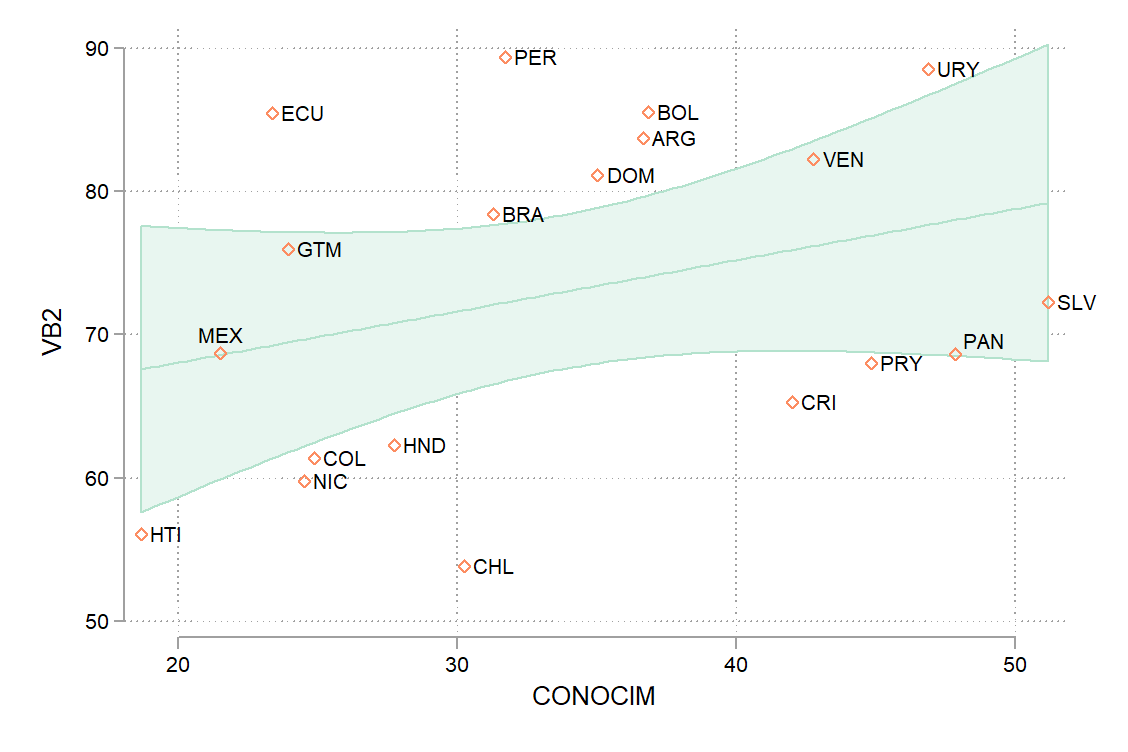
\includegraphics[width=.30\linewidth]{figures/conocim-part}}
  \subfloat[PROT3]{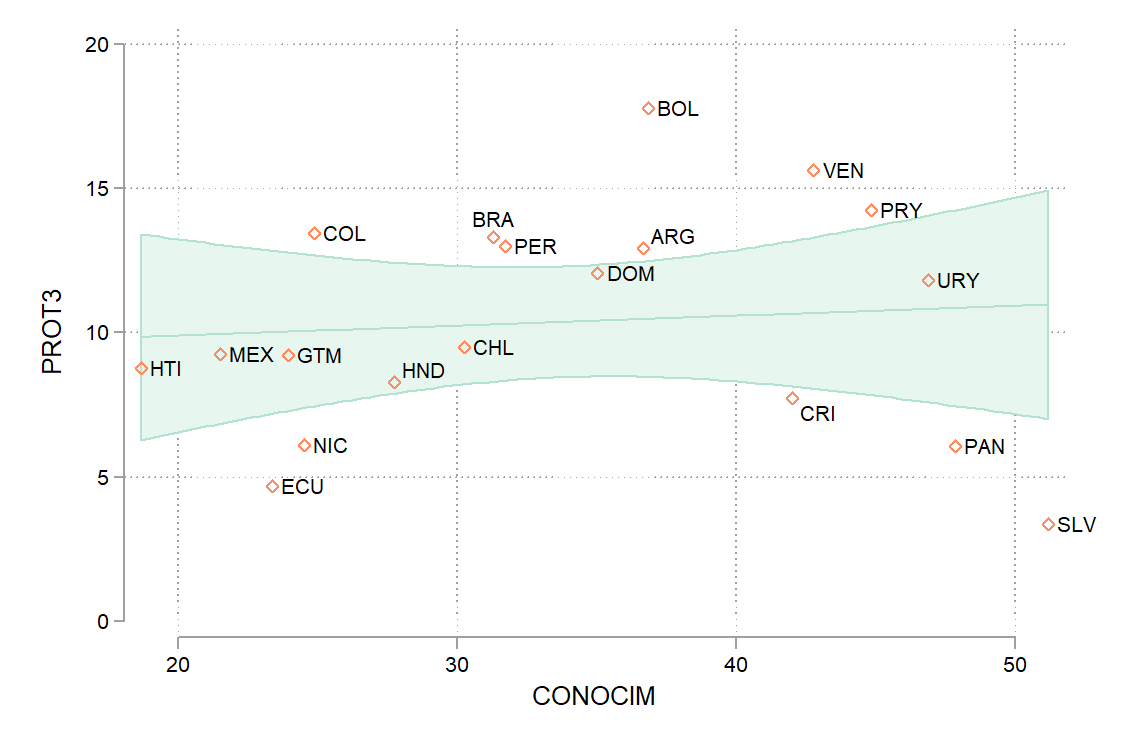
\includegraphics[width=.30\linewidth]{figures/conocim-prot}}
  \subfloat[EFF1]{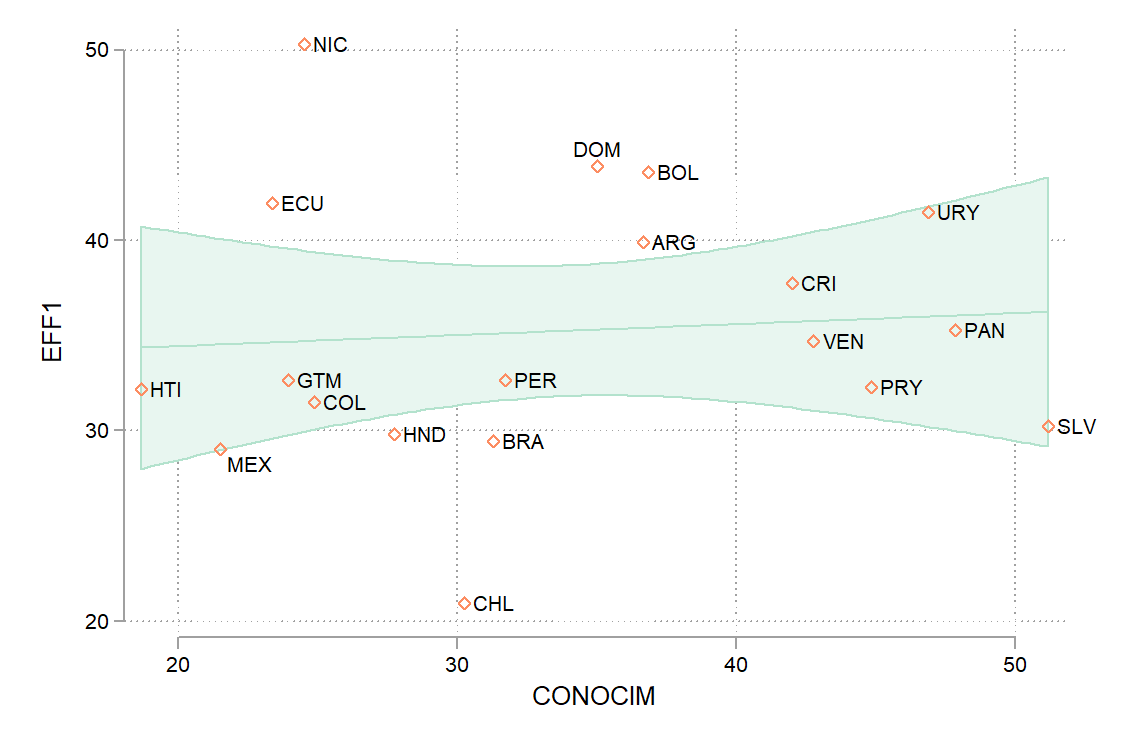
\includegraphics[width=.30\linewidth]{figures/conocim-eff}}\\
   \subfloat[VB10]{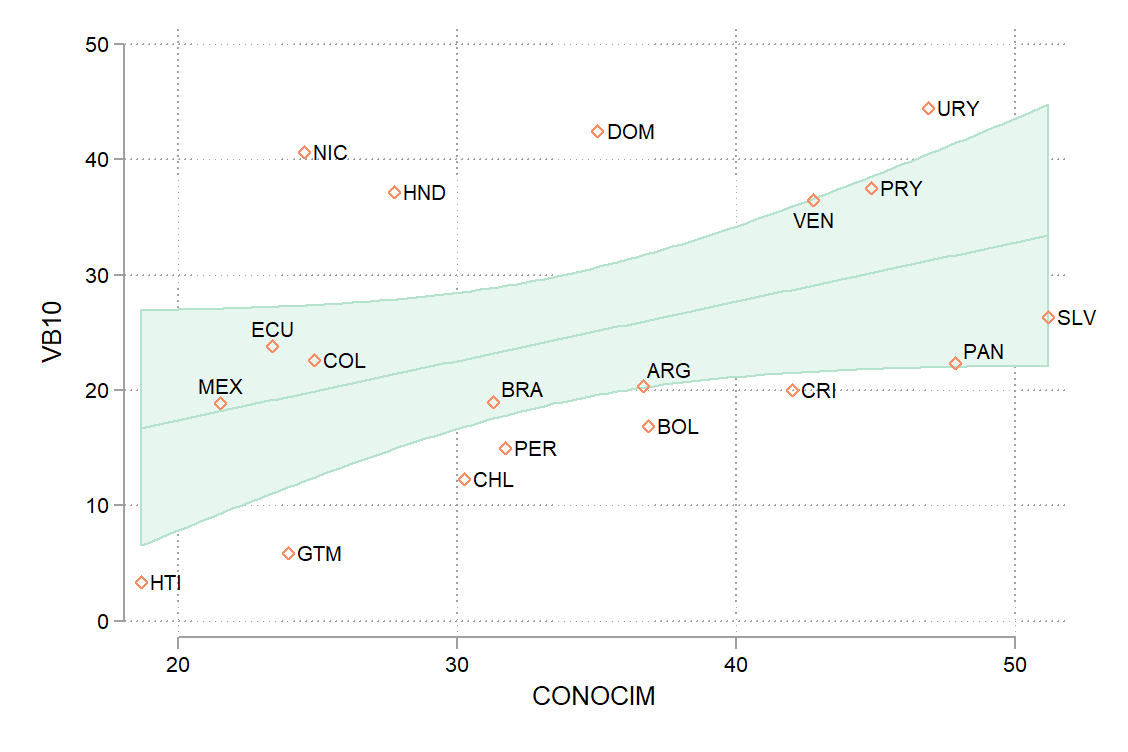
\includegraphics[width=.30\linewidth]{figures/conocim-id-part}}
   \subfloat[POL1]{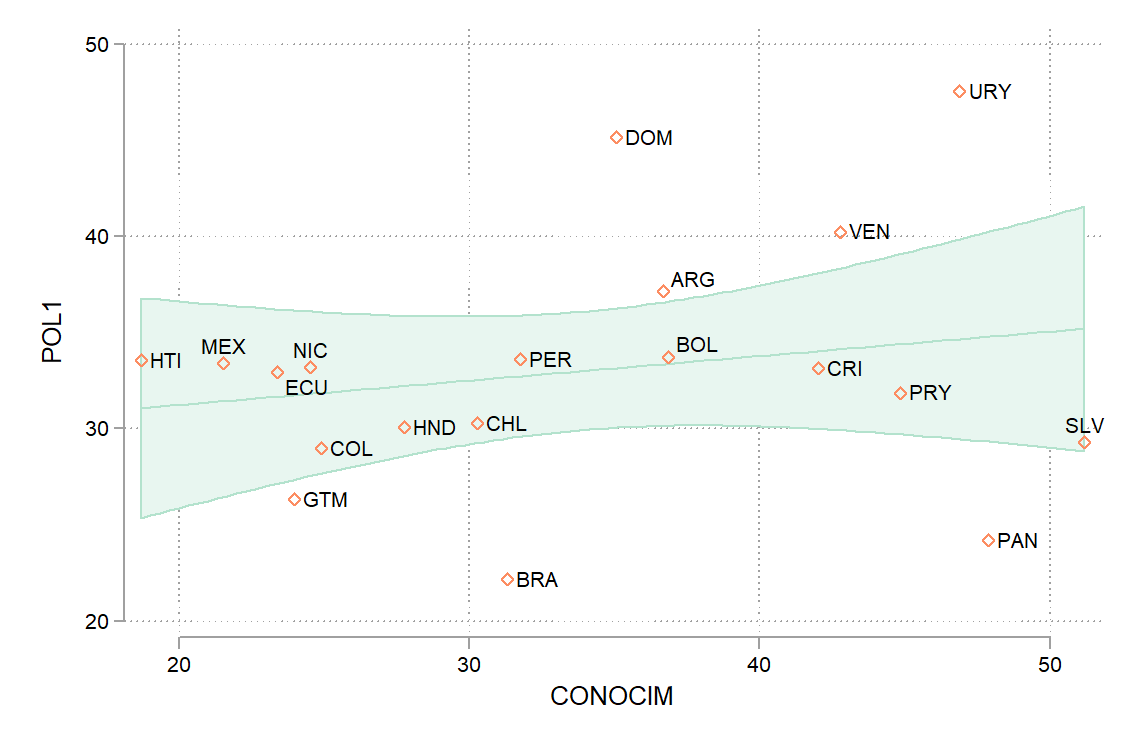
\includegraphics[width=.30\linewidth]{figures/conocim-int}}
   \subfloat[GI0]{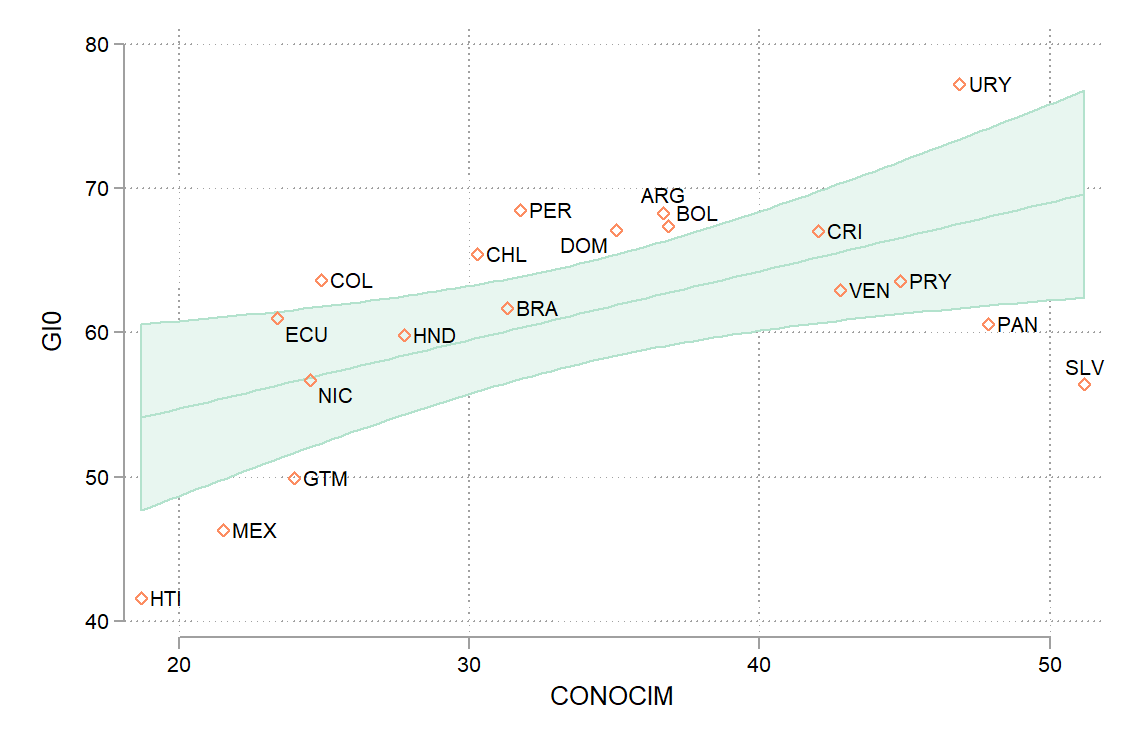
\includegraphics[width=.30\linewidth]{figures/conocim-medios}}
  %% \caption{}
  %% \label{fig:fullfig}
  \\ \smallskip\noindent\scriptsize Fuente: Elaboración propia con datos del Barómetro de las Américas 2016/17 por LAPOP, \href{https://www.vanderbilt.edu/lapop/}{\textcolor{blue}{www.LapopSurveys.org}}.
\end{figure*}

\subsection[Modelos logísticos agrupados de un nivel] {Modelos logísticos agrupados de un nivel}

\justify{A continuación, en la tabla 2, se presentan los resultados de los modelos con regresiones logísticas agrupadas para cada una de las variables dependientes utilizadas. En los modelos se presentan los coeficientes beta y los errores estándar. Posteriormente, para las variables significativas se presentan en el texto la razón de momios (odds ratio, OR) y sus respectivos intervalos de confianza al 95\%.}

\begin{table*}[h]
  \centering
  \fontfamily{ppl}\selectfont
   \smallskip\noindent\small Tabla 1 (Parte 1/2) \\ Regresiones logísticas agrupadas para participación y compromiso político, América Latina 2016/17  \\~\\
  \begin{tabular}{l c c c c c c}
    \toprule
     & VB2 & PROT3 & EFF1 & VB10 & POL1 & GI0 \\ \midrule
    \multicolumn{7}{c}{Control} \\ \midrule
    \multirow{2}{*}{Q1} & -0,105$^\star$$^\star$$^\star$ & 0,125$^\star$$^\star$$^\star$ & 0,036 & 0,243$^\star$$^\star$$^\star$ & 0,184$^\star$$^\star$$^\star$ & 0,040 \\
    & {\scriptsize (0,028)} & {\scriptsize (0,039)} & {\scriptsize (0,024)} & {\scriptsize (0,029)} & {\scriptsize (0,027)} & {\scriptsize (0,025)} \\ 
    \multirow{2}{*}{Q2} & & & & & & \\
    & & & & & & \\
    \multirow{2}{*}{UR} & & & & & & \\
    & & & & & & \\ \midrule
    \multicolumn{7}{c}{Sofisticación} \\ \midrule
    \multirow{2}{*}{CONOC.} & & & & & & \\
    & & & & & & \\ \midrule
    \multicolumn{7}{c}{Países} \\ \midrule
    \multirow{2}{*}{ARG} & & & & & & \\
    & & & & & & \\
    \multirow{2}{*}{BOL} & & & & & & \\
    & & & & & & \\
    \multirow{2}{*}{BRA} & & & & & & \\
    & & & & & & \\
    \multirow{2}{*}{COL} & & & & & & \\
    & & & & & & \\
    \multirow{2}{*}{CRI} & & & & & & \\
    & & & & & & \\
    \multirow{2}{*}{ECU} & & & & & & \\
    & & & & & & \\
    \multirow{2}{*}{SLV} & & & & & & \\
    & & & & & & \\
    \multirow{2}{*}{GTM} & & & & & & \\
    & & & & & & \\ \bottomrule
  \end{tabular}
  \\~\\ \smallskip\noindent\scriptsize $\dagger$ $p \leq 0,1$ | $\star$ $p \leq 0,05$ | $\star\star$ $p \leq 0,01$ | $\star\star\star$ $p \leq 0,001$  \\ Nota: Se reportan coeficientes $\beta$ y errores estándar entre paréntesis. Se aplica un ajuste para modelos con muestras complejas con el estimador de varianza Taylor linealizado considerando los estratos de la muestra ({\itshape strata}), las unidades primarias de muestreo ({\itshape PSUs}) y el factor de expansión muestral estandarizado para comparabilidad entre países ({\itshape weight1500}). Se reporta McKelvey y Zavoina $R^2$. \\ Fuente: Elaboración propia con datos del Barómetro de las Américas 2016/17 por LAPOP, \href{https://www.vanderbilt.edu/lapop/}{\textcolor{blue}{www.LapopSurveys.org}}.
\end{table*}

\begin{table*}[h]
  \centering
  \fontfamily{ppl}\selectfont
   \smallskip\noindent\small Tabla 1 (Parte 2/2) \\ Regresiones logísticas agrupadas para participación y compromiso político, América Latina 2016/17 \\~\\
  \begin{tabular}{l c c c c c c}
    \toprule
     & VB2 & PROT3 & EFF1 & VB10 & POL1 & GI0 \\ \midrule
    \multicolumn{7}{c}{Países} \\ \midrule
    \multirow{2}{*}{HTI} & & & & & & \\
    & & & & & & \\ 
    \multirow{2}{*}{HND} & & & & & & \\
    & & & & & & \\
    \multirow{2}{*}{MEX} & & & & & & \\
    & & & & & & \\
    \multirow{2}{*}{NIC} & & & & & & \\
    & & & & & & \\
    \multirow{2}{*}{PAN} & & & & & & \\
    & & & & & & \\
    \multirow{2}{*}{PRY} & & & & & & \\
    & & & & & & \\
    \multirow{2}{*}{PER} & & & & & & \\
    & & & & & & \\ 
    \multirow{2}{*}{DOM} & & & & & & \\
    & & & & & & \\ 
    \multirow{2}{*}{URY} & & & & & & \\
    & & & & & & \\
    \multirow{2}{*}{VEN} & & & & & & \\
    & & & & & & \\ \midrule
    \multirow{2}{*}{Constante} & & & & & & \\
    & & & & & & \\ \midrule
    $N$ & & & & & & \\
    $N$ ({\itshape strata}) & & & & & & \\
    $N$ ({\itshape PSUs}) & & & & & & \\ \midrule
    {\itshape Pseudo}-$R^2$ & & & & & & \\ \bottomrule
  \end{tabular}
  \\~\\ \smallskip\noindent\scriptsize $\dagger$ $p \leq 0,1$ | $\star$ $p \leq 0,05$ | $\star\star$ $p \leq 0,01$ | $\star\star\star$ $p \leq 0,001$  \\ Nota: Se reportan coeficientes $\beta$ y errores estándar entre paréntesis. Se aplica un ajuste para modelos con muestras complejas con el estimador de varianza Taylor linealizado considerando los estratos de la muestra ({\itshape strata}), las unidades primarias de muestreo ({\itshape PSUs}) y el factor de expansión muestral estandarizado para comparabilidad entre países ({\itshape weight1500}). Se reporta McKelvey y Zavoina $R^2$. \\ Fuente: Elaboración propia con datos del Barómetro de las Américas 2016/17 por LAPOP, \href{https://www.vanderbilt.edu/lapop/}{\textcolor{blue}{www.LapopSurveys.org}}.
\end{table*}

\justify{El primer modelo muestra que el conocimiento político aumenta la probabilidad de participar electoralmente (OR = 1,262; CI95\% = 1,225; 1,302), lo mismo ocurre con la edad (OR = 1,054; CI95\% = 1,052; 1,057). Por otra parte, ser hombre (OR = 0,900; CI95\% = 0,852; 0,951) y vivir en zonas urbanas (OR = 0,842; CI95\% = 0,785; 0,904) disminuyen las probabilidades de participar electoralmente.}

\justify{El conocimiento político también aumenta la probabilidad de participar en protestas (OR = 1,032; CI95\% = 1,250; 1,359), al igual que ser hombre (OR = 1,133; CI95\% = 1,050; 1,223). La edad tiende a disminuir la probabilidad de participar en protestas (OR = 0,992; CI95\% = 0,990; 0,994), mientras que el tipo de residencia no resulta ser una variable significativa (p = 0,560).}

\justify{En el caso de la eficacia política el conocimiento funciona de forma inversa ya que disminuye sus probabilidades (OR = 0,911; CI95\% = 0,887; 0,936). Lo mismo ocurre con residir en zonas urbanas (OR = 0,875; CI95\% = 0,825; 0,928). La edad, por otro lado, aumenta la eficacia política (OR = 1,007; CI95\% = 1,005; 1,008), mientras que el sexo no resulta significativo (p = 0,131).}

\justify{Para la identificación partidaria el conocimiento vuelve a funcionar de forma directa aumentando las probabilidades de que una persona sienta cercanía con un partido (OR = 1,232; CI95\% = 1,197; 1,268), lo mismo sucede con ser hombre (OR = 1,275; CI95\% = 1,205; 1,350) y con la edad (OR = 1,018; CI95\% = 1,016; 1,019). Por otro lado, vivir en zonas urbanas disminuye la identificación con partidos (OR = 0,821; CI95\% = 0,767; 0,878).}

\justify{El conocimiento político también aumenta el interés en la política (OR = 1,485; CI95\% = 1,443; 1,528), al igual que ser hombre (OR = 1,202; CI95\% = 1,140; 1,267). Por otra parte, la edad disminuye las probabilidades de tener interés en la política (OR = 0,989; CI95\% = 0,987; 0,990) y la zona de residencia no emerge como variable estadísticamente significativa (p = 0,752).}

\justify{Por último, el conocimiento político aumenta la probabilidad de consumir medios (OR = 1,327; CI95\% = 1,292; 1,364), al igual que la edad (OR = 1,024; CI95\% = 1,023; 1,026) y vivir en zonas urbanas (OR = 1,343; CI95\% = 1,261; 1,429). El sexo no es una variable estadísticamente significativa en este modelo (p = 0,115).}

\justify{En el gráfico 3 se muestran los efectos marginales promedio por país para los distintos modelos. Las {\itshape dummies} de países sugieren que para participación electoral existen considerables efectos de país en todos los casos en distintas proporciones, aunque en todos se verifica mayor propensión a votar que en Chile.}

\begin{figure*}[h!]
\captionsetup[subfigure]{labelformat=empty}
  \centering
  \smallskip\noindent\small Figura 3 \\ Efectos marginales promedio de participación y compromiso político, América Latina 2016/17
  \subfloat[VB2]{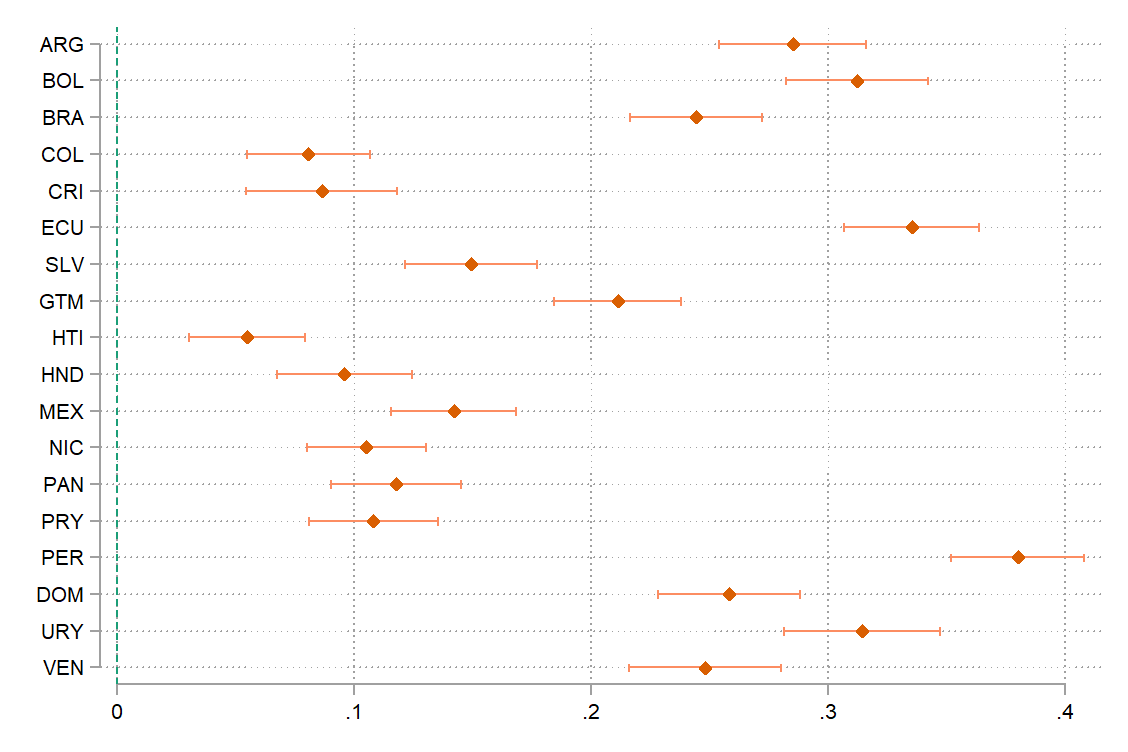
\includegraphics[width=.30\linewidth]{figures/logit-part}}
  \subfloat[PROT3]{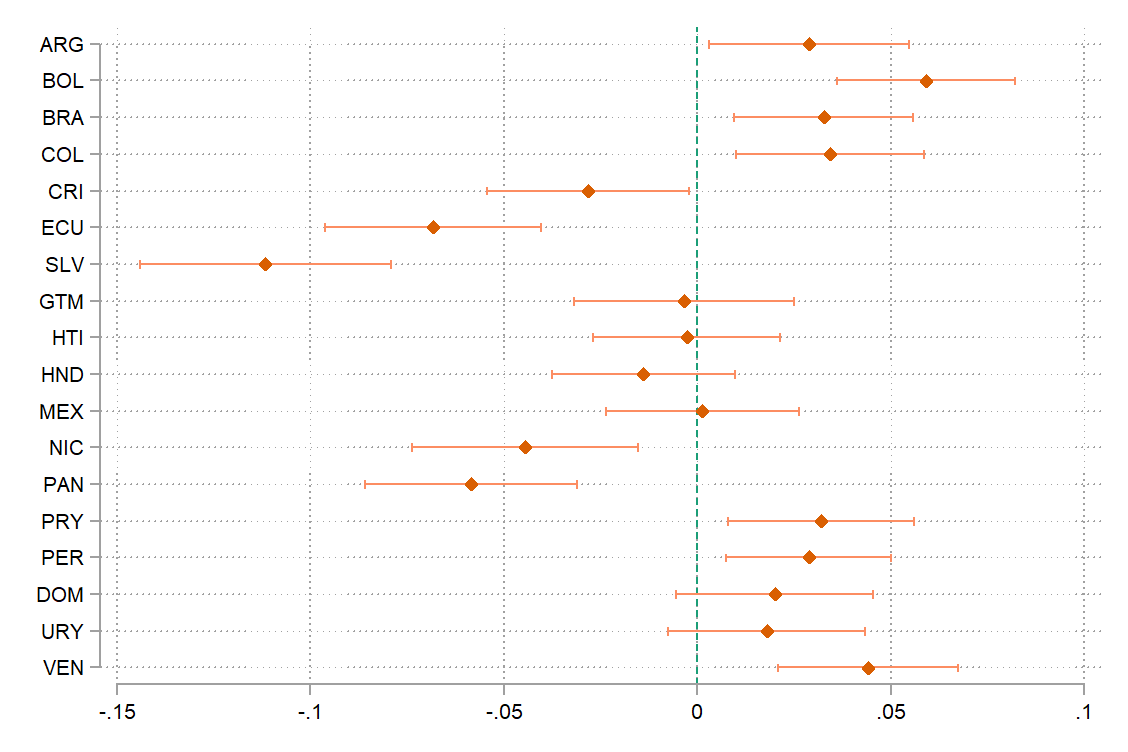
\includegraphics[width=.30\linewidth]{figures/logit-prot}}
  \subfloat[EFF1]{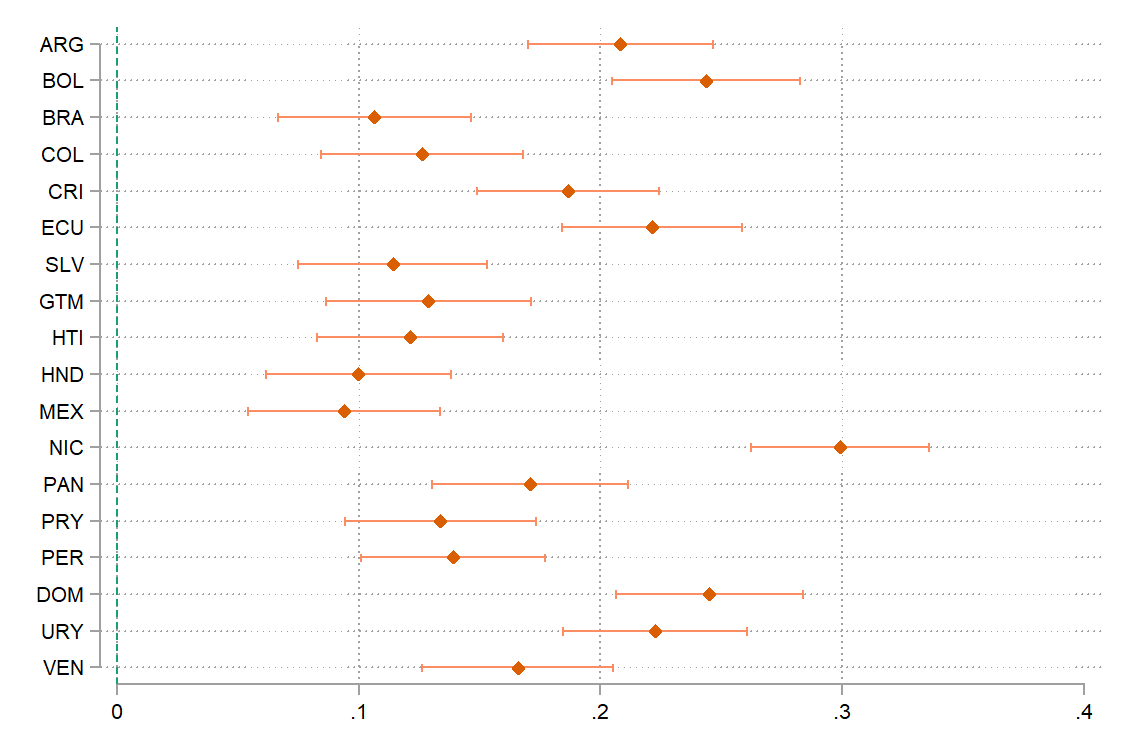
\includegraphics[width=.30\linewidth]{figures/logit-eff}}\\
   \subfloat[VB10]{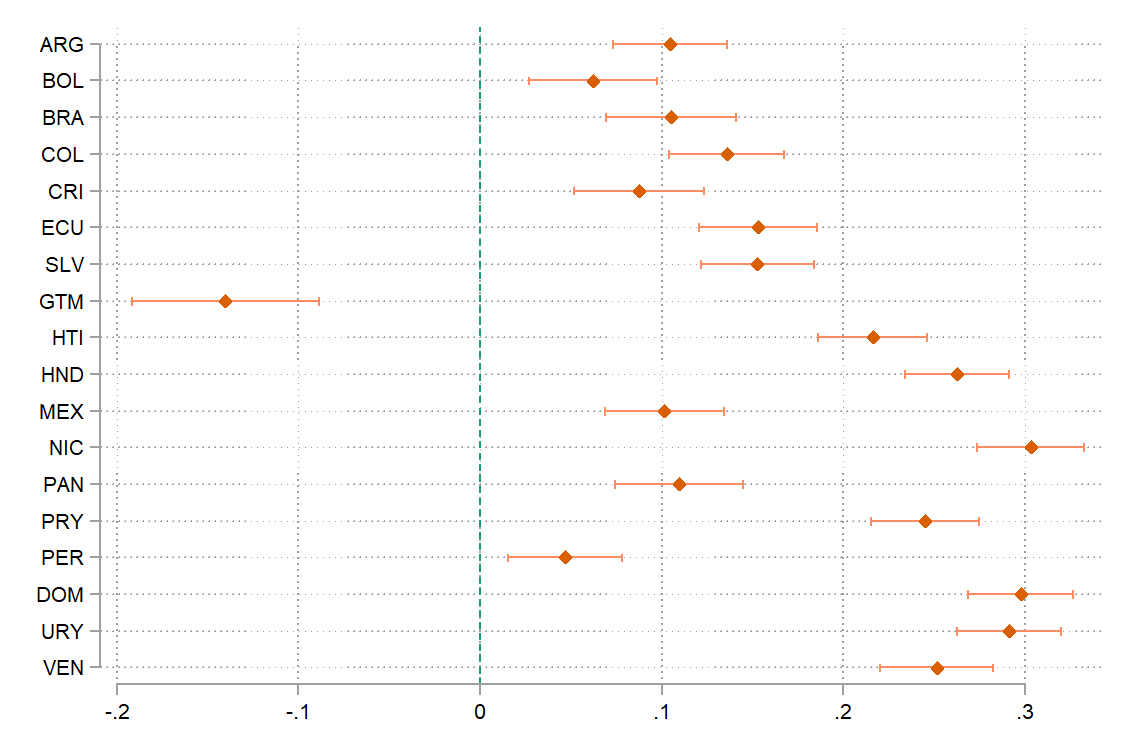
\includegraphics[width=.30\linewidth]{figures/logit-id-part}}
   \subfloat[POL1]{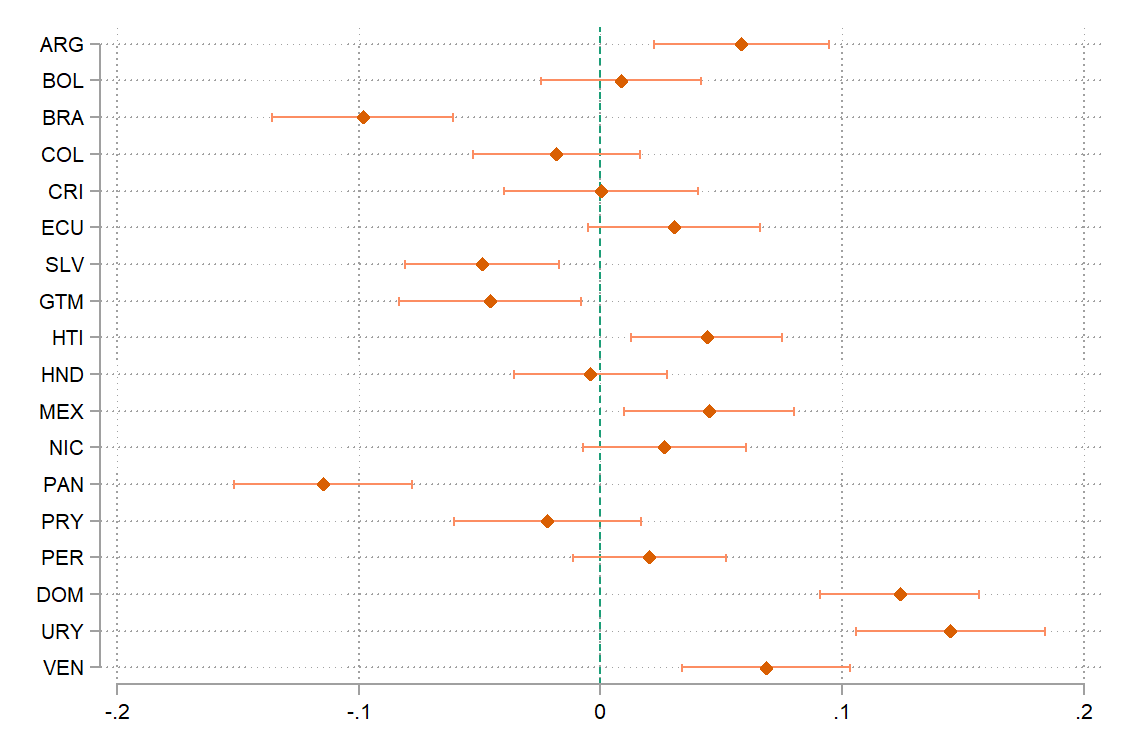
\includegraphics[width=.30\linewidth]{figures/logit-int}}
   \subfloat[GI0]{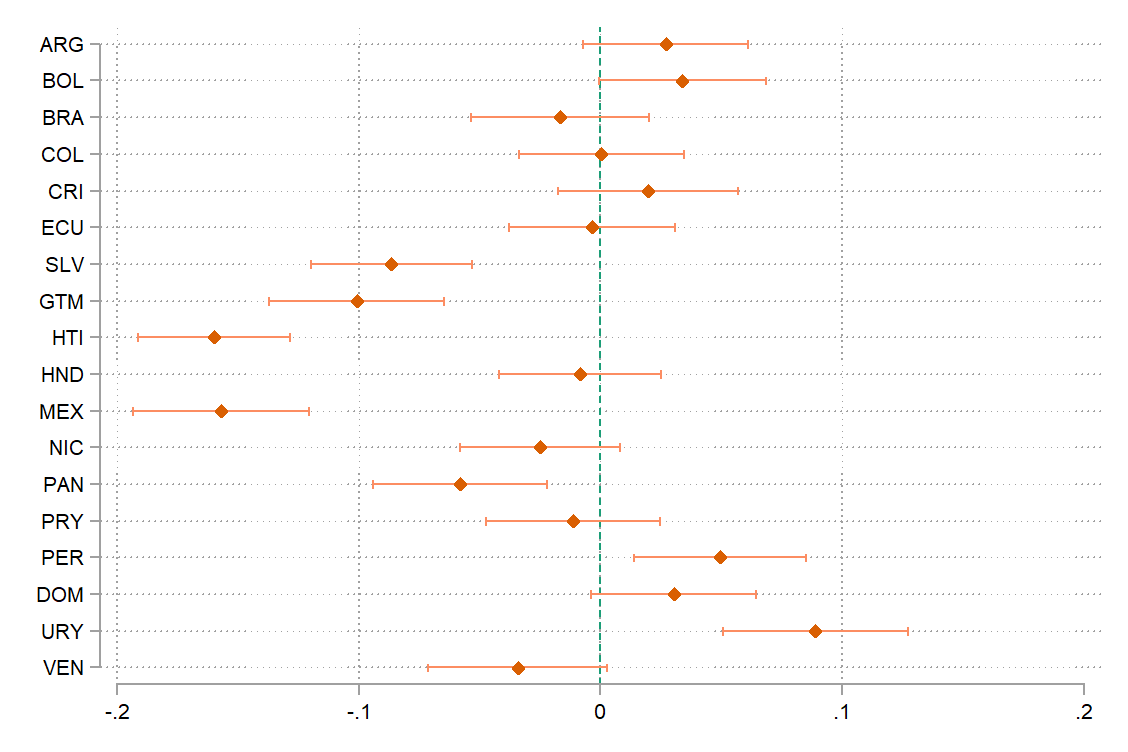
\includegraphics[width=.30\linewidth]{figures/logit-medios}}
  \\ \smallskip\noindent\scriptsize Nota: Se utiliza Chile como país de referencia. \\ Fuente: Elaboración propia con datos del Barómetro de las Américas 2016/17 por LAPOP, \href{https://www.vanderbilt.edu/lapop/}{\textcolor{blue}{www.LapopSurveys.org}}.
\end{figure*}

\justify{Con respecto a la manifestación, los casos que tienden a protestar más que Chile son: Argentina, Bolivia, Brasil, Colombia, Paraguay, Perú y Venezuela. Los países que tienen menor propensión son: Costa Rica, Ecuador, El Salvador, Nicaragua y Panamá. No existen diferencias significativas con Guatemala (p = 0,816), Haití (p = 0,827), Honduras (p = 0,249), México (p = 0,914), República Dominicana (p = 0,122) y Uruguay (p = 0,164).}

\justify{Por otro lado, en eficacia política también se advierten efectos de país en todos los casos en distintas proporciones y, al igual que en la participación electoral, todos verifican mayor propensión que Chile. Lo mismo sucede en el caso de la identificación partidaria, con la única excepción de que Guatemala es el único caso donde la identificación tiende a ser menor que en Chile.}

\justify{El interés en la política tiene distintos efectos por país. En Argentina, Haití, México, República Dominicana, Uruguay y Venezuela hay mayor propensión a presentar interés en la política que en Chile. Por otra parte, Brasil, El Salvador, Guatemala y Panamá tienen menor propensión. No se advierten diferencias estadísticamente significativas con Bolivia (p = 0,611), Colombia (p = 0,300), Costa Rica (p = 0,990), Ecuador (p = 0,092), Honduras (p = 0,797), Nicaragua (p = 0,122), Paraguay (p = 0,268) y Perú (p = 0,209).}

\justify{Por último, solo en dos países hay mayor propensión al consumo de medios que en Chile: Perú y Uruguay. De forma contraria, El Salvador, Guatemala, Haití, México y Panamá presentan menor propensión. El resto de los países no presenta diferencias estadísticamente significativas: Argentina (p = 0,122), Bolivia (p = 0,054), Brasil (p = 0,373), Colombia (p = 0,986), Costa Rica (p = 0,304), Ecuador (p = 0,840), Honduras (p = 0,623), Nicaragua (p = 0,139), Paraguay (p = 0,544), República Dominicana (p = 0,082) y Venezuela (p = 0,069).}

\justify{A continuación, en el gráfico 4, se pueden apreciar los efectos del conocimiento político en cada modelación: participación electoral (p = 0,000), en protestas (p = 0,000), eficacia política (p = 0,000), identificación partidaria (p = 0,000), interés en la política (p = 0,000) y consumo de medios (p = 0,000). Solo para eficacia el efecto es inverso: a mayor conocimiento político, menor percepción de que a los gobernantes les interesa lo que piensa la ciudadanía.}

\begin{figure*}[h!]
\captionsetup[subfigure]{labelformat=empty}
  \centering
  \smallskip\noindent\small Figura 4 \\ Márgenes predictivos de conocimiento político para participación y compromiso político, América Latina 2016/17
  \subfloat[VB2]{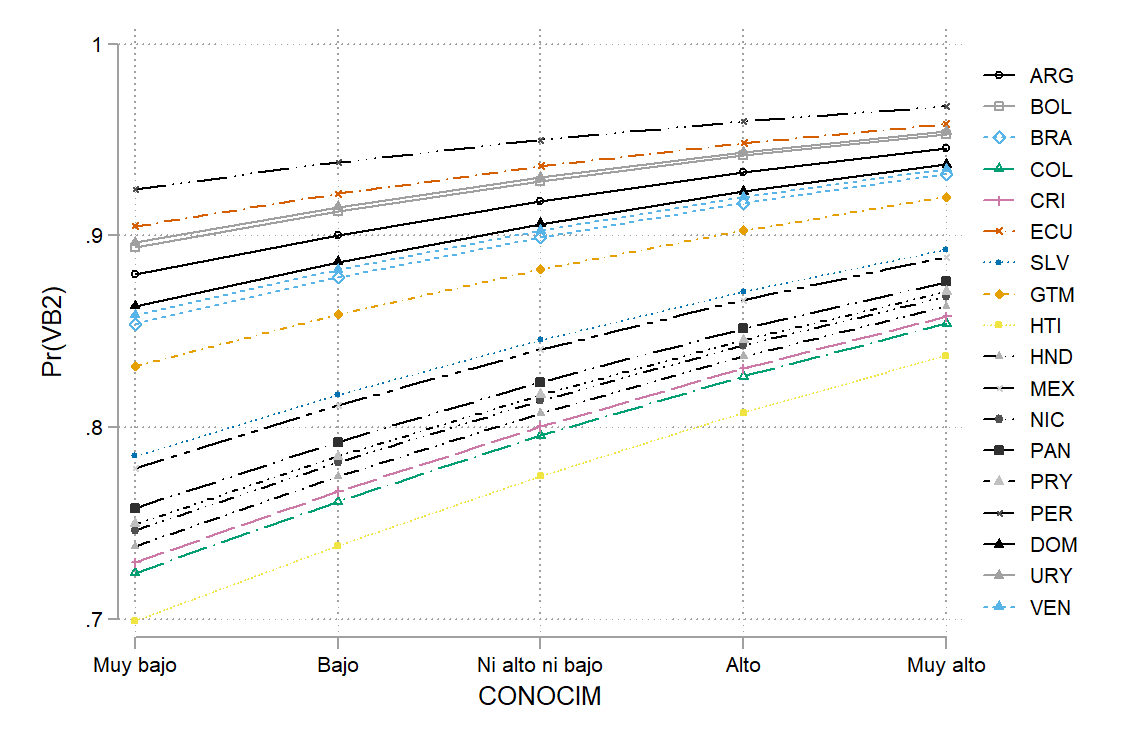
\includegraphics[width=.30\linewidth]{figures/margin-part}}
  \subfloat[PROT3]{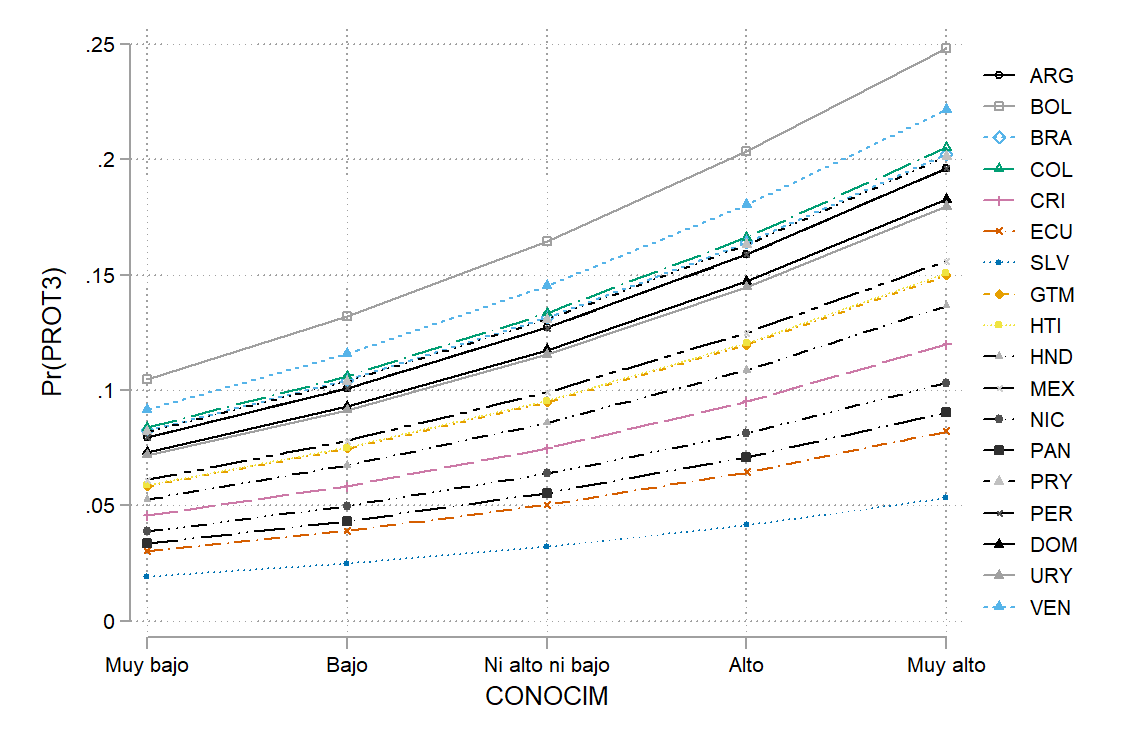
\includegraphics[width=.30\linewidth]{figures/margin-prot}}
  \subfloat[EFF1]{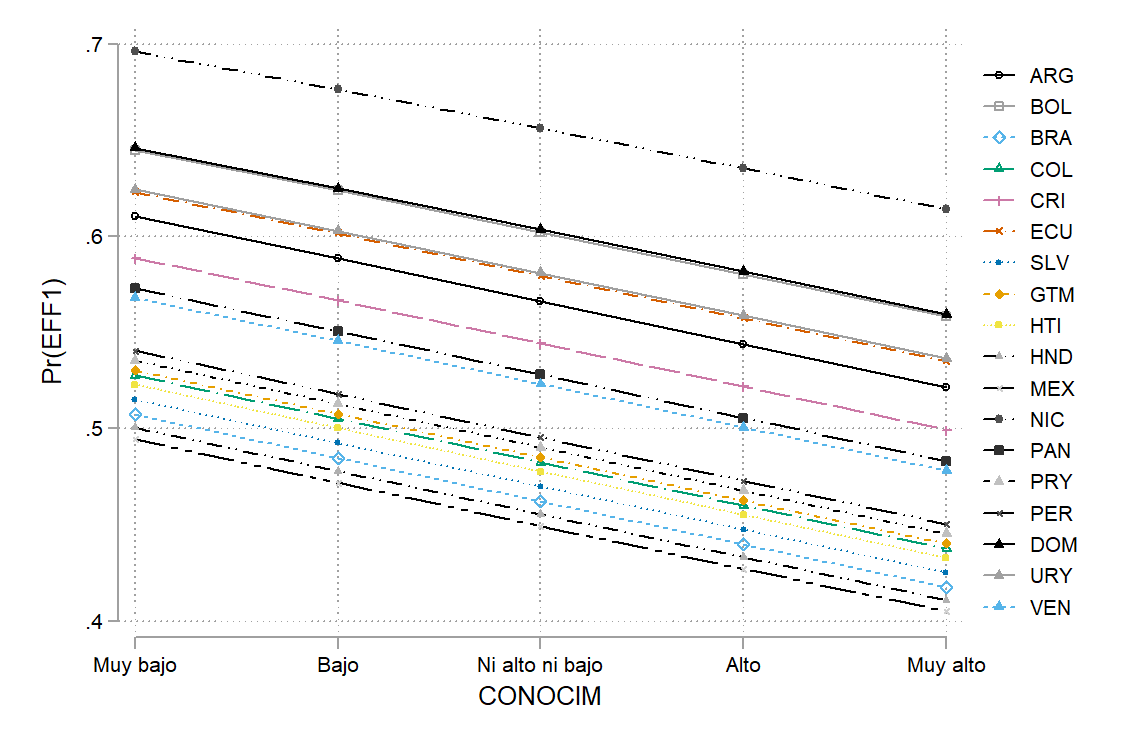
\includegraphics[width=.30\linewidth]{figures/margin-eff}}\\
   \subfloat[VB10]{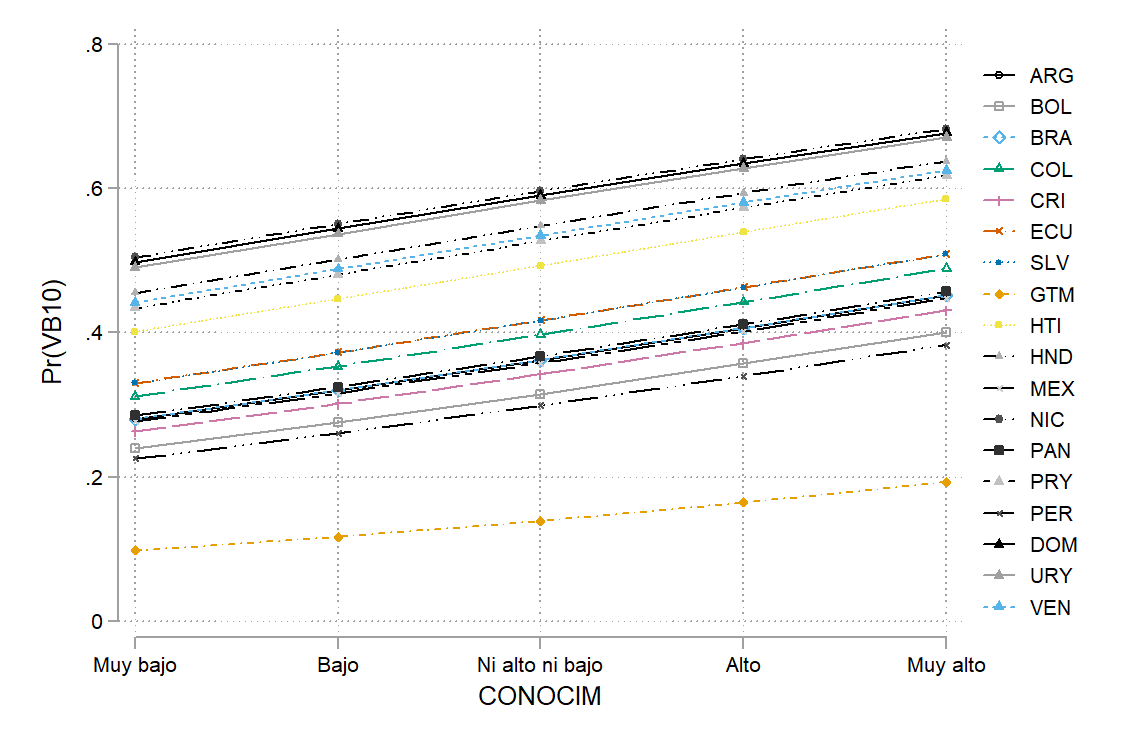
\includegraphics[width=.30\linewidth]{figures/margin-id-part}}
   \subfloat[POL1]{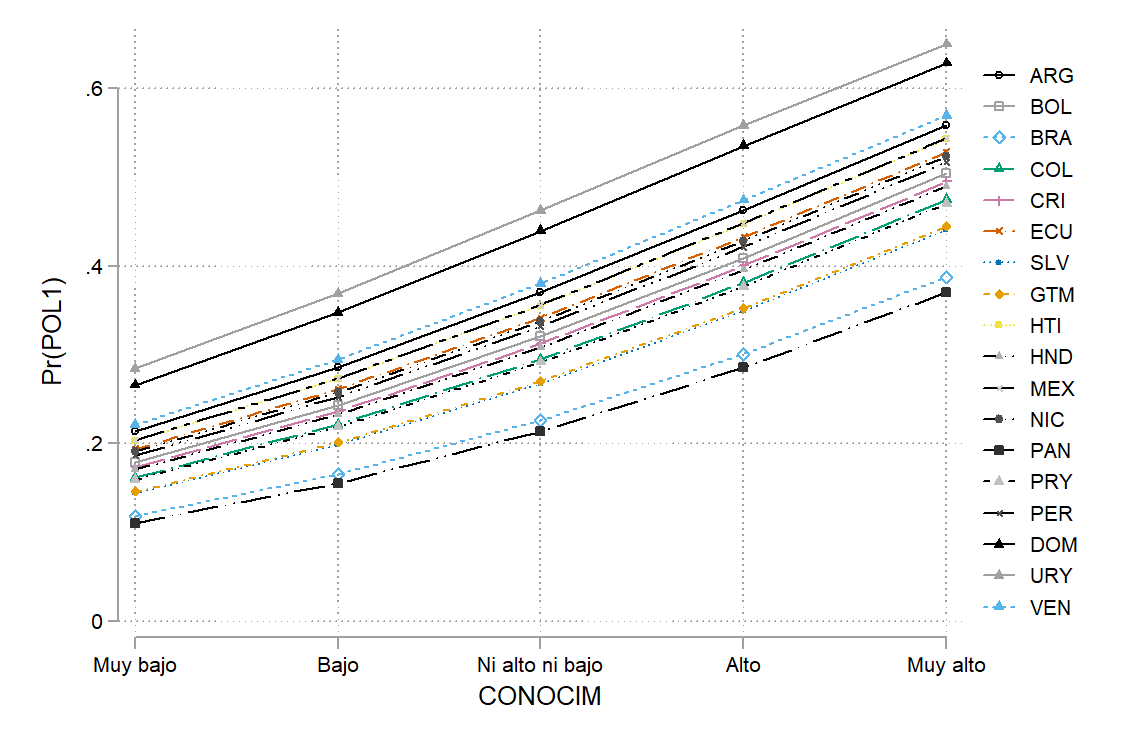
\includegraphics[width=.30\linewidth]{figures/margin-int}}
   \subfloat[GI0]{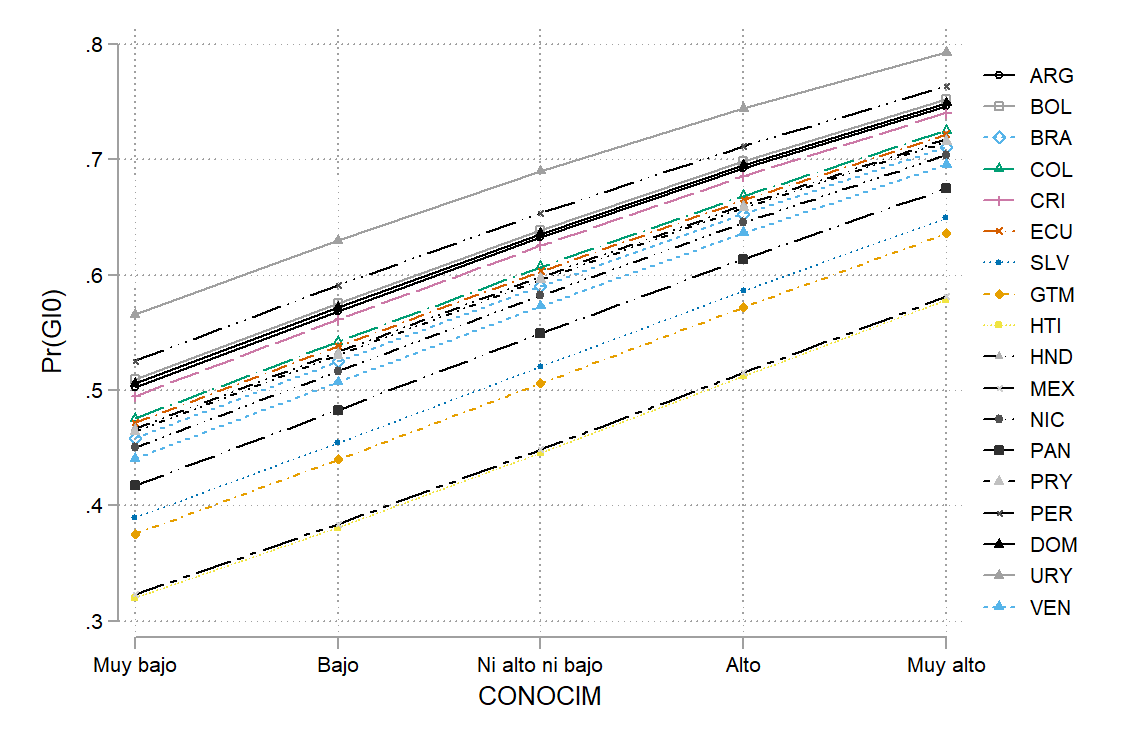
\includegraphics[width=.30\linewidth]{figures/margin-medios}}
  \\ \smallskip\noindent\scriptsize Nota. Se utiliza Chile como país de referencia. Otras variables {\itshape céteris páribus}. \\ Fuente: Elaboración propia con datos del Barómetro de las Américas 2016/17 por LAPOP, \href{https://www.vanderbilt.edu/lapop/}{\textcolor{blue}{www.LapopSurveys.org}}.
\end{figure*}

\subsection[Modelos de efectos mixtos de dos niveles] {Modelos de efectos mixtos de dos niveles}

\justify{A continuación, en la tabla 3, se presentan los modelos de efectos mixtos. En el modelo de participación electoral se puede apreciar que el conocimiento político aumenta su probabilidad de ocurrencia (OR = 1,262; CI95\% = 1,225; 1,299), de la misma forma que la edad (OR = 1,054; CI95\% = 1,052; 1,056). De forma opuesta, ser hombre (OR = 0,921; CI95\% = 0,871; 0,974) y vivir en zonas urbanas (OR = 0,842; CI95\% = 0,791; 0,897) disminuyen la participación electoral. El modelo de efectos mixtos ratifica los resultados del modelo logístico, de hecho, la razón de momios de las variables significativas varía en promedio solo un 0,58\%.}

\begin{table*}[h]
  \centering
  \fontfamily{ppl}\selectfont
   \smallskip\noindent\small Tabla 3 \\ Regresiones logísticas de efectos mixtos para participación y compromiso político, América Latina 2016/17 \\~\\
  \begin{tabular}{l c c c c c c}
    \toprule
     & VB2 & PROT3 & EFF1 & VB10 & POL1 & GI0 \\ \midrule
    \multicolumn{7}{c}{Control} \\ \midrule
    \multirow{2}{*}{Q1} & & & & & \\
    & & & & & & \\ 
    \multirow{2}{*}{Q2} & & & & & & \\
    & & & & & & \\
    \multirow{2}{*}{UR} & & & & & & \\
    & & & & & & \\ \midrule
    \multicolumn{7}{c}{Sofisticación} \\ \midrule
    \multirow{2}{*}{CONOC.} & & & & & & \\
    & & & & & & \\ \midrule
    \multirow{2}{*}{Constante} & & & & & & \\
    & & & & & & \\ \midrule
    \multicolumn{7}{c}{Efectos aleatorios} \\ \midrule    
    \multirow{2}{*}{País} & & & & & & \\
    & & & & & & \\ \midrule
    LL & & & & & & \\ \midrule
    $N$ & & & & & & \\ \midrule
    AIC & & & & & & \\
    BIC & & & & & & \\ \bottomrule
  \end{tabular}
  \\~\\ \smallskip\noindent\scriptsize $\dagger$ $p \leq 0,1$ | $\star$ $p \leq 0,05$ | $\star\star$ $p \leq 0,01$ | $\star\star\star$ $p \leq 0,001$  \\ Nota: Se reportan coeficiente beta y errores estándar entre paréntesis. Para los efectos aleatorios el anidamiento en segundo nivel es por país y se indica la significancia de la prueba de contraste entre efectos fijos y aleatorios.\\ Fuente: Elaboración propia con datos del Barómetro de las Américas 2016/17 por LAPOP, \href{https://www.vanderbilt.edu/lapop/}{\textcolor{blue}{www.LapopSurveys.org}}.
\end{table*}

\justify{En el modelo de participación en protestas el conocimiento político también tiene un efecto positivo (OR = 1,306; CI95\% = 1,256; 1,358), lo mismo ocurre con ser hombre (OR = 1,157; CI95\% = 1,074; 1,246). La edad tiende un efecto inverso: a mayor edad, menores probabilidades de manifestar (OR = 0,992; CI95\% = 0,990; 0,995). La zona de residencia, al igual que en el modelo logístico agrupado, no es estadísticamente significativa (p = 0,912). La variación promedio de las probabilidades de las variables significativas entre el modelo logístico y el de efectos mixtos es de un 9,56\%, principalmente porque el conocimiento político aumenta en un 26,55\%.}

\justify{Por otra parte, al igual que en el modelo logístico, el conocimiento político disminuye la eficacia (OR = 0,913; CI95\% = 0,890; 0,936), lo mismo aplica para residir en zonas urbanas (OR = 0,896; CI95\% = 0,849; 0,946). La edad, en cambio, aumenta la eficacia (OR = 1,006; CI95\% = 1,005; 1,008). El sexo del individuo no resulta ser una variable estadísticamente significativa (p = 0,140). También se mantienen los mismos patrones del modelo logístico con una variación mínima, solo de un 0,84\%.}

\justify{Con respecto a la identificación partidaria, el conocimiento aumenta sus probabilidades (OR = 1,232; CI95\% = 1,198; 1,267), lo mismo ocurre en el modelo logístico. Otras variables que son predictores de identificación con los partidos son ser hombre (OR = 1,299; CI95\% = 1,230; 1,372) y la edad (OR = 1,017; CI95\% = 1,016; 1,019), patrones que también se advierten en la regresión logística. Vivir en zonas urbanas, por otra parte, disminuye las probabilidades de identificación partidaria (OR = 0,820; CI95\% = 0,771; 0,872). La variación entre el modelo logístico y el de efectos mixtos es solo de un 0,42\% para las variables significativas.}

\justify{El conocimiento político también aumenta el interés en la política (OR = 1,490; CI95\% = 1,451; 1,530), también ocurre este efecto con ser hombre (OR = 1,225; CI95\% = 1,166; 1,287). Por otro lado, mientras la edad disminuye el interés (OR = 0,989; CI95\% = 0,987; 0,990), vivir en zonas urbanas o rurales resulta irrelevante (p = 0,519). Estos son los mismos resultados que arrojó el modelo logístico para interés en la política. Se advierte una variación promedio de un 0,75\%.}

\justify{Finalmente, el conocimiento político también constituye un predictor de consumo de medios (OR = 1,331; CI95\% = 1,298; 1,365), al igual que la edad (OR = 1,024; CI95\% = 1,022; 1,026) y vivir en zonas urbanas (OR = 1,319; CI95\% = 1,250; 1,392). El sexo no resulta ser una variable significativa (p = 0,076). Se advierten los mismos patrones que en el modelo logístico y la variación promedio de las variables significativas es solo de un 0,50\% negativo ya que la razón de momios de la residencia disminuye en un 1,79\% con respecto al modelo logístico.}

\justify{A continuación, en el gráfico 5, se grafica el logaritmo de las razones de momios por país para evaluar el efecto del conocimiento político en cada modelo de efectos mixtos: participación electoral (p = 0,000), participación en protestas (p = 0,000), eficacia política (p = 0,000), identificación partidaria (p = 0,000), interés en la política (p = 0,000) y consumo de medios (p = 0,000). El efecto es inverso solo en eficacia política, al igual que en los modelos logísticos agrupados de un nivel.}

\section[Discusi\'on] {{\normalfont Discusi\'on}}

%%%%%%%%%%%%%%%%%%%%%%%%%%%%%%%%%%%%%%%%%%%%%%%%%%

\section{{\normalfont Referencias}}

\begin{list}{}%
{\leftmargin=1em \itemindent=-1em}

\item{\small Maillet, A., Gonz\'alez-Bustamante, B., {\itshape \&} Olivares, A. (2016). ?`Puerta giratoria? An\'alisis de la circulaci\'on p\'ublico-privada en Chile (2000-2014). {\itshape Serie de Documentos de Trabajo PNUD-Desigualdad}, (7),  1-40.}
\end{list}

%%%%%%%%%%%%%%%%%%%%%%%%%%%%%%%%%%%%%%%%%%%%%%%%%%

\end{document}
